\chapter{Chrétiens et musulmans au XXe siècle}

\mn{Marie Carmen}

\section{Quelques références bibliographiques}

\begin{itemize}
    \item 
 
Abitbol
Michel, Histoire du Maroc Paris, Perrin, coll « Tempus », 2014
    \item 
Bessis
Sophie, Histoire de la Tunisie de Carthage à nos jours, Paris, Taillandier, 2019
    \item 
Bonin
Hubert, L'empire colonial français de l'histoire aux héritages XX e XXI e siècles, Paris, Armand Colin, « Collection U », 2018
    \item 
Bouchène
Abderrahmane, Peyroulou Jean Pierre, et al dir Histoire de l'Algérie à la période coloniale 1830 1962 Paris, La Découverte,
2012
    \item 
Chouikha
Larbi et Gobe Eric Histoire de la Tunisie depuis l’indépendance, Paris, La Découverte, coll « Repères », 2015
    \item 
Droz
Bernard, Histoire de la décolonisation au XX e siècle, Paris, Le Seuil, « L'Univers historique », 2006
    \item 
Georgeon
François, Vatin Nicolas et Veinstein Gilles dir Dictionnaire de l’Empire ottoman Paris, Fayard, 2015 2 e édition en poche aux
éditions du CNRS, coll « Biblis », 2022
    \item 
Hourani
Albert, Histoire des peuples arabes Paris, Seuil, coll « Points », 1993
    \item 
Phan
Bernard, Colonisation et décolonisation ..(XVI e XX e siècle Paris, Presses Universitaires de France, « Quadrige », 2017
\end{itemize}

\section{Quelques dates importantes (1)}

\begin{itemize}

\item Campagne d'Egypte : 
    \item 
 
Mai
juin 1830 : expédition d’Alger


 
    \item 
Mai 1837 : traité de Tafna
    \item 
1839 : rupture du traité de Tafna
    \item 
Novembre 1848 : Algérie devient «
territoire français »
    \item 
Avril 1863 :
Senatus Consulte sur la propriété foncière
    \item 
Juillet 1865 :
Senatus Consulte sur l’état des personnes et la naturalisation
en Algérie

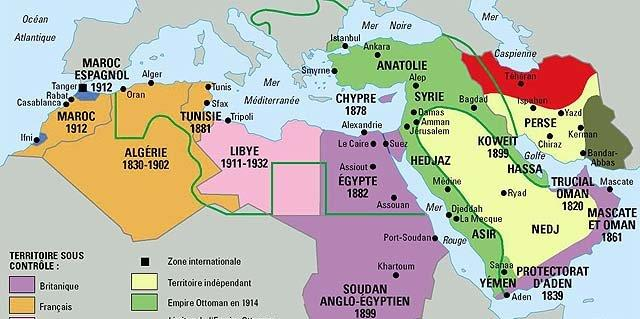
\includegraphics[width=0.8\textwidth]{HistoireIslamMediterranee/Images/Colonie.jpg}
    \item 
1881 : Tunisie devient protectorat français (Traité du Bardo : mai 1881)
    \item 
1912 : Maroc devient protectorat français (Traité de Fès : mars 1912)

\item Indépendance du Maroc : 3 mars 1956
\item
Indépendance de la Tunisie : 20 mars 1956
\item
Indépendance de l’Algérie : 3 juillet 1962
\end{itemize}


\mn{ Séance du 04/04/2023 Note de Jean François Normand Période contemporaine
Marie-Carmen Smyrnelis} 

\section{Approche historique}
De toute époque, il y a des périodes et des modes de colonisation.
Plus particulièrement au 19e 
Colonisation européenne du Maghreb dans un contexte de regard biaisé sur les autres (en se pensant en supériorité).
\paragraph{Expédition de la France en 1798}
 : incursion de 3 ans de l’Europe au cœur du monde musulman. Perçus comme des envahisseurs per les Égyptiens. Une mission à la fois militaire et scientifique.

\paragraph{1815}
Après 1815, la France perd la plupart de ses colonies au bénéfice de l’Angleterre. En 1914 le pays occupe 25\% de la planète.
Il n’y a pas que des convictions politiques dans cet investissement. Le coût de l’entretien des colonies devient rapidement un sujet de débat, l’alternative ayant pu être une logique de présence via des comptoirs.
Une logique de concurrence s’installe entre puissances pour conquérir de nouveaux espaces.
\paragraph{Algérie}
Pour la France l’expansion reprend en 1830 avec l’Algérie sans qu’il y ait une stratégie manifeste pour la Méditerranée.  Le Maroc était sous protectorat. L’Algérie et la Tunisie payaient un tribut à l’empire Ottoman. Un « dey » payait une redevance à l’empire – régions barbaresques soumis à la piraterie dans un contexte d’autonomie grandissant du fait de leur éloignement d’Istanbul.


\includegraphics[width=0.8\textwidth]{HistoireIslamMediterranee/Images/algérie.jpg}

Sur un différend au sujet du non-paiement d’une livraison de blé, un affrontement diplomatique dégénère entre le Dey d’Alger et la France de Charles X. 
\begin{itemize}
    \item Expédition française quitte Toulon le 18 mai 1830 et débarque à Alger le 14 juin. 
\end{itemize}
Abdication du Dey. L’expédition a aussi des motivations économiques de la part de marchands français cherchant d’autres débouchés commerciaux.
\paragraph{Absence de réaction de l’empire ottoman. }
Résistances des tribus locales galvanisées par l’émir Abd el Kader.
Situation figée avec hésitations sur la stratégie à suivre jusqu’en 1834. Négociations avec l’émir Abd el Kader (Traité de Tafna 1837).

En 1839, lancement d’une politique d’occupation totale (direction Général Bugeaud) dans un contexte de crise économique sévère dans toute l’Europe.

\paragraph{En 1848, L’Algérie devient territoire français}
  s’ensuit une vague d’immigration européenne constituée de réfugiés politiques, économiques. Conditions très difficiles pour les populations autochtones (expropriation, famines) mais aussi pour les colons qui ne sont pas adaptés à ce nouvel environnement.
Utopie d’une société moralisée malgré l’envoi de personnes dont on ne veut plus (brigands, révolutionnaires,…)


\section{Senatus Consulte}

\begin{quote}
    Extrait du
Senatus Consulte sur l’état des
personnes et la naturalisation en Algérie (1865)
 
Article premier
L'indigène musulman est Français ; néanmoins il continuera à être régi par la loi musulmane. Il peut être admis à servir dans
le s armées de terre et
de mer. il peut être appelé à des fonctions et emplois civils en Algérie. Il peut, sur sa demande, être admis à jouir des dro its de citoyen français ; dans
ce cas il est régi par les lois civiles et politiques de la France.
 
Article 2
L'indigène
israëlite est Français ; néanmoins il continue à être régi par son statut personnel. Il peut être admis à servir dans les armées de ter re et de
mer. il peut être appelé à des fonctions et emplois civils en Algérie. Il peut, sur sa demande, être admis à jouir des droits de citoyen français ; dans ce
cas il est régi par la loi française.
 
Article 3
L'étranger qui justifie de trois années de résidence en Algérie peut être admis à jouir de tous les droits de citoyen français.
 
Article 4
La qualité de citoyen français ne peut être obtenue, conformément aux articles 1, 2 et 3 du présent sénatus
consulte, qu'à l'âge de vingt et un ans
accomplis ; elle est conférée par décret impérial rendu en conseil d'Etat.
\end{quote}
\paragraph{L’indigène musulman devient français}
 et peut jouir des droits de citoyens français et doit renoncer alors aux lois musulmanes pour suivre les lois et la juridiction française. L’étranger non indigène peut bénéficier du même statut après 3 années de résidence.
Discours critiques sur les discriminations entre catégories de français. L’exercice de la religion musulmane n’est plus libre.

\paragraph{Maroc / Tunisie}
Au Maroc (1912) et en Tunisie (Traité du Bardo 1880), nous avons d’autres statuts : celui de protectorat. On semble y respecter la singularité du pays car il y a un chef local (sultan marocain, Bey tunisien) mais c’est bien la France qui régit le territoire.


 \paragraph{Réforme dans les provinces musulmanes de l’empire ottoman}

Courant réformiste qui souhaite revenir sur les fondamentaux de l’islam pour retrouver la grandeur passée. 
\begin{Ex}[Abduh]
Exemple de M.Abduh qui prône une combinaison des deux approches entre ouverture à l’occident et retour aux sources.
Courant moderniste radicaux qui veulent suivre le modèle occidental
\end{Ex}


\paragraph{Émergence d’un nationalisme arabe}
 (prend sa forme après 1908) chez les chrétiens arabes qui dénoncent la légitimité du sultan ottoman et dénonce les occupations étrangères.
Après le conflit 1ère guerre mondiale traité des mandats à la France (Syrie-Liban) et l’Angleterre (Palestine, trans-jordanie, Irak, Koweit). Ce qui renforce les nationalismes arabes, les élites étant formés dans les écoles occidentales. Le vrai nationalisme émerge dans la suite de la première guerre en réaction aux investissements et sacrifices consentis aux efforts de guerre par les territoires colonisés
Parti nationaliste tunisien Destour (1920), néo Destour Bourguiba (1930).
Mouvement des Frères musulmans (1928)
Fondation de la Ligue arabe en 1948 pour resserrer les liens entre les pays arabes.

\paragraph{L’Europe n’est plus le centre du monde.
}
Guerre froide.
Conférence de Bandung (1955) accélère la décolonisation
Maroc et Tunisie (1956) avec retour du souverain sur le trône
Algérie (1962) après une guerre de plus de 8 ans

